% =====================================================================
%  BSMI 風力發電預測 — 七專案總覽簡報 (Beamer)
%  編譯：xelatex 風力發電預測_總覽簡報.tex   (需兩次以生成目錄/頁碼)
%  依賴：ctex, beamer, booktabs, amsmath, graphicx, tikz
%  圖片以相對路徑引用；請將本檔置於 D:\ML_wind\ 根目錄編譯。
% =====================================================================
\documentclass[aspectratio=169,11pt]{beamer}

\usepackage{ctex}                 % 中文（建議 xelatex）
\usepackage{amsmath,amssymb}
\usepackage{booktabs}
\usepackage{graphicx}
\usepackage{array}
\usepackage{tikz}
\usetikzlibrary{arrows.meta,positioning}

% ---------- 主題與配色 ----------
\usetheme{default}
\usecolortheme{whale}
\useinnertheme{circles}
\definecolor{accent}{RGB}{30,95,168}
\definecolor{accent2}{RGB}{13,143,111}
\definecolor{fam2}{RGB}{139,63,176}
\definecolor{warn}{RGB}{181,70,42}
\setbeamercolor{structure}{fg=accent}
\setbeamercolor{frametitle}{bg=accent,fg=white}
\setbeamercolor{title}{fg=white}
\setbeamertemplate{navigation symbols}{}
\setbeamertemplate{footline}[frame number]
\setbeamerfont{frametitle}{size=\large,series=\bfseries}
\setbeamertemplate{itemize items}[circle]

\newcommand{\best}[1]{\textcolor{accent2}{\textbf{#1}}}
\newcommand{\fam}[1]{\textcolor{accent}{\small[家族一]}\,#1}
\renewcommand{\arraystretch}{1.15}

% ---------- 標題頁資訊 ----------
\title{\textbf{BSMI 風力發電預測：七專案整合總覽}}
\subtitle{原始資料 → 品質控制 → 虛擬出力 → 特徵 → 方法 → 驗證 → 結果}
\author{風能機器學習專案}
\date{BSMI 100\,m 測風塔 · 2016-03 $\sim$ 2021-10（66 個月）}

\begin{document}

% ===================== 封面 =====================
\begin{frame}[plain]
  \titlepage
  \begin{center}\footnotesize
  278{,}600 筆有效 10 分鐘紀錄 \quad|\quad 容量因數 $\approx$ 45\% \quad|\quad LightGBM 主力 \quad|\quad 全部可重現
  \end{center}
\end{frame}

% ===================== 目錄 =====================
\begin{frame}{本簡報結構}
  \tableofcontents
\end{frame}

% =====================================================================
\section{0. 總覽與專案地圖}
% =====================================================================
\begin{frame}{七專案分類表}
  \scriptsize
  \begin{tabular}{lllll}
    \toprule
    \textbf{專案} & \textbf{來源檔} & \textbf{驗證/QC} & \textbf{機型} & \textbf{出力單位}\\
    \midrule
    PW & BSMI\_10min & 自建 01 獨立 QC & $\sim$8\,MW & 正規化 0–1\\
    PW\_Integrated & BSMI\_10min & 自建 01 獨立 QC & $\sim$8\,MW & 正規化 0–1\\
    PW\_Interval & BSMI\_10min & 自建 01 獨立 QC & $\sim$8\,MW & 正規化 0–1\\
    power\_forecast\_interval\_ge & BSMI\_10min & 自建 01 獨立 QC & $\sim$8\,MW & 正規化 0–1\\
    power\_forecast（根） & BSMI\_10min & 直接信 \texttt{is\_valid} & $\sim$8\,MW & 正規化 0–1\\
    power\_interval\_forecast\_cl & BSMI\_10min & 直接信 \texttt{is\_valid} & $\sim$8\,MW & 正規化 0–1\\
    \textcolor{fam2}{\textbf{advanced\_forecasting}} & \textcolor{fam2}{BSMI\_10min+turb} & 直接信 \texttt{is\_valid} & \textcolor{fam2}{\textbf{NREL 5\,MW}} & \textcolor{fam2}{\textbf{絕對 kW/MW}}\\
    \bottomrule
  \end{tabular}
  \vspace{4pt}
  \begin{block}{兩大家族}
  \footnotesize
  \textbf{家族一}（6 個）：虛擬 $\sim$8\,MW、\textbf{正規化 0–1}，結論對機型穩健。\quad
  \textbf{家族二}（1 個）：NREL 5\,MW 官方曲線、\textbf{絕對 MW/MWh}，另併湍流特徵。
  \end{block}
\end{frame}

\begin{frame}{關鍵概念：「區間」有兩個意思}
  \begin{columns}[T]
    \column{0.5\textwidth}
      \begin{block}{時間的區間（窗口 / 能量）}
      預測未來 $[t{+}1,t{+}H]$ 的\textbf{平均或總量}。\\
      「未來這段時間\underline{總共}發多少電？」\\[3pt]
      $\Rightarrow$ PW\_Interval、interval\_ge（\textbf{系統 A}）
      \end{block}
    \column{0.5\textwidth}
      \begin{block}{不確定性的區間（機率）}
      對某預測值給\textbf{可信範圍} p10–p90。\\
      「這一刻\underline{多不確定}？」\\[3pt]
      $\Rightarrow$ interval\_cl、advanced（\textbf{系統 B}）
      \end{block}
  \end{columns}
  \vspace{6pt}
  \centering
  \textbf{系統 A 管「一天大概發多少」，系統 B 管「每一刻有多少把握」。}
\end{frame}

% =====================================================================
\section{整理框架（六階段）}
% =====================================================================
\begin{frame}{建議的整理框架：由五階段擴為六階段}
  \centering
  \begin{tikzpicture}[
    node distance=3.5mm,
    st/.style={rectangle,rounded corners,draw=accent,very thick,fill=accent!5,
               minimum height=1.05cm,text width=1.9cm,align=center,font=\scriptsize},
    ar/.style={-{Stealth[length=2mm]},accent,thick}]
    \node[st](a){\textbf{①}\\原始資料\\+ QC};
    \node[st,right=of a,fill=accent2!10,draw=accent2](b){\textbf{②★新增}\\虛擬出力\\（物理）};
    \node[st,right=of b](c){\textbf{③}\\特徵工程};
    \node[st,right=of c](d){\textbf{④}\\預測方法};
    \node[st,right=of d](e){\textbf{⑤}\\建模與\\驗證};
    \node[st,right=of e](f){\textbf{⑥}\\結果與\\應用};
    \draw[ar](a)--(b);\draw[ar](b)--(c);\draw[ar](c)--(d);\draw[ar](d)--(e);\draw[ar](e)--(f);
  \end{tikzpicture}
  \vspace{6pt}
  \begin{block}{為何補這兩階段（給教授的重點）}
  \footnotesize
  \begin{itemize}
    \item \textbf{② 虛擬出力是核心前提}：塔\underline{無實測發電量}，$Y$ 由功率曲線＋密度修正推得——獨立成階段才能誠實交代 $Y$ 來源與「為何用正規化」。
    \item \textbf{① QC 是可信度地基}：七專案差異之一即「自建獨立 QC」vs「直接信 \texttt{is\_valid}」，顯性化才知每個數字站在什麼資料品質上。
  \end{itemize}
  \end{block}
\end{frame}

% =====================================================================
\section{① 原始資料與品質控制}
% =====================================================================
\begin{frame}{① 原始資料與品質控制}
  \begin{columns}[T]
    \column{0.52\textwidth}
    \textbf{BSMI 100\,m 離岸測風塔}
    \begin{itemize}\footnotesize
      \item 1\,Hz 逐秒，2016-03 $\sim$ 2021-10（66 月）
      \item 4 高度風速 100E/100W/69W/38W\,m
      \item 2 風向 97/35\,m；溫、濕、壓 $\to$ 空氣密度
      \item \textbf{塔本身無實測發電量}
      \item 聚合為 \texttt{BSMI\_10min}；湍流表 \texttt{BSMI\_turb}
    \end{itemize}
    \column{0.48\textwidth}
    \textbf{四重獨立 QC}（家族一）
    \begin{itemize}\footnotesize
      \item 去重 + 連續 10 分鐘網格
      \item 物理範圍檢查（風速/溫/濕/壓/密度）
      \item 感測器凍結偵測（連續 $\ge$1\,h 定值）
      \item 四高度一致性、風向向量長度
    \end{itemize}
  \end{columns}
  \vspace{4pt}
  \centering\footnotesize
  \begin{tabular}{cccc}
    \toprule
    網格點 & 有觀測 & \best{通過 QC 有效} & 建模用($\ge$4 m/s)\\
    \midrule
    295{,}997 & 279{,}055 & \best{278{,}612 (99.8\%)} & 211{,}564\\
    \bottomrule
  \end{tabular}
\end{frame}

% =====================================================================
\section{② 虛擬出力建模（物理層）}
% =====================================================================
\begin{frame}{② 虛擬出力：空氣密度修正 + 功率曲線}
  \textbf{IEC 61400-12-1 空氣密度修正}（源於 $P\propto\rho U^3$）：
  \[ v_{\text{eff}} = U_{100}\left(\frac{\rho}{\rho_0}\right)^{1/3},\qquad \rho_0=1.225\ \text{kg/m}^3 \]
  \begin{columns}[T]
    \column{0.5\textwidth}
    \textbf{家族一：$\sim$8\,MW 正規化曲線}
    \[ P=\operatorname{interp}(v_{\text{eff}};\mathbf{u}_{\text{pc}},\mathbf{p}_{\text{pc}})\in[0,1] \]
    {\scriptsize 切入 3、額定 $\sim$12、切出 25 m/s}
    \column{0.5\textwidth}
    \textbf{家族二：NREL 5\,MW 官方曲線}
    \[ P_{\text{kW}}=\operatorname{interp}(v_{\text{eff}};\mathbf{u}_{\text{NREL}},\mathbf{p}_{\text{NREL}}) \]
    {\scriptsize 額定 5000\,kW（11.4 m/s），$E=\sum P\,\Delta t$}
  \end{columns}
  \vspace{3pt}
  \textbf{敏感度立方模型}\;$P=\dfrac{u^3-u_{\text{in}}^3}{u_{\text{r}}^3-u_{\text{in}}^3}$（$u_{\text{in}}{\le}u{<}u_{\text{r}}$）\quad
  \textbf{輪轂外推}\;$U_{\text{hub}}=U_{100}(h/100)^{\alpha}$
\end{frame}

\begin{frame}{② 站點資源評估（物理層的直接產物）}
  \begin{columns}[c]
    \column{0.42\textwidth}
    \footnotesize
    \begin{tabular}{lc}
      \toprule 指標 & 數值\\ \midrule
      容量因數 CF & \best{45.0\%}\\
      等效滿載時數 & 3{,}942–3{,}949 h/年\\
      最佳月(12月) CF & 70.8\%\\
      最差月(8月) CF & 20.7\%\\
      最保守機型 CF & 31\%（仍優質）\\
      \bottomrule
    \end{tabular}
    \vspace{4pt}
    \begin{block}{誠實界線}\scriptsize
    出力是物理推算、\textbf{非實測}；家族一用正規化 $P$ 讓結論對機型穩健。
    \end{block}
    \column{0.58\textwidth}
    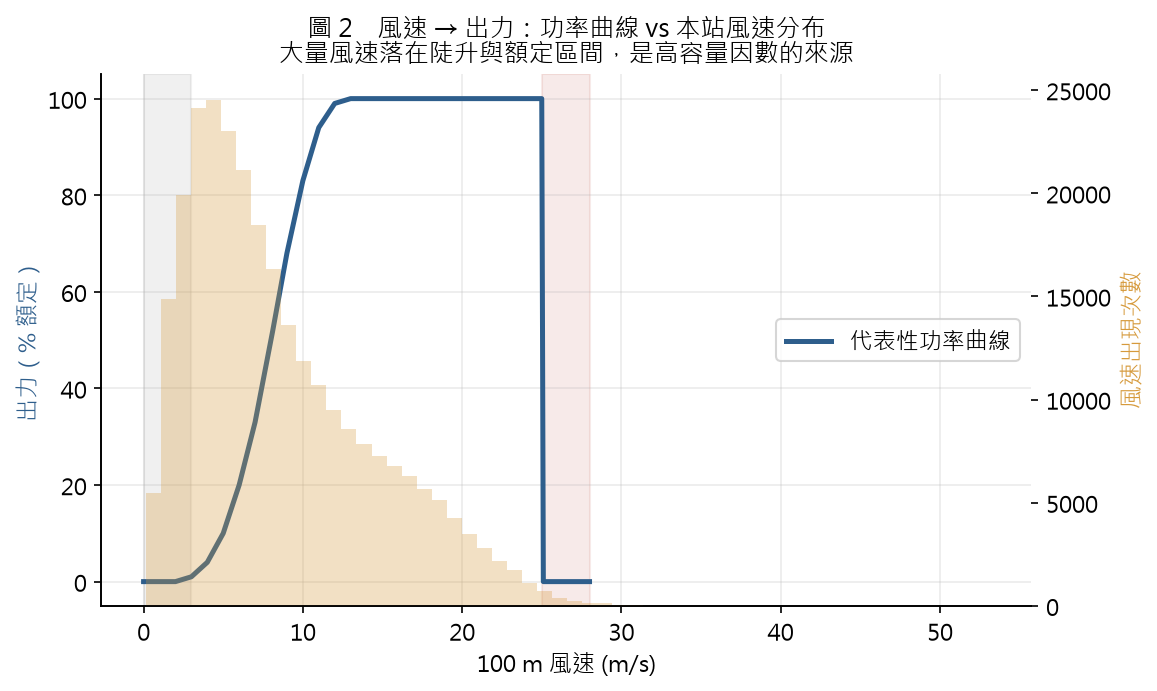
\includegraphics[width=\linewidth]{ml_project/power_forecast/figures/res2_power_curve.png}
  \end{columns}
\end{frame}

% =====================================================================
\section{③ 特徵工程}
% =====================================================================
\begin{frame}{③ 特徵工程（44 特徵 · 無洩漏）}
  \begin{columns}[T]
    \column{0.55\textwidth}
    \footnotesize
    \textbf{三類特徵}
    \begin{itemize}
      \item \textbf{當前氣象態}：多高度風速、TI、陣風因子、風向 sin/cos 與 $\sigma$、溫濕壓、風切 $\alpha$、密度、當前 $P$
      \item \textbf{時間動態}：lag（$t{-}10\ldots180$ 分）、滾動均值/標準差/min/max/\textbf{趨勢斜率}、變化率 diff
      \item \textbf{週期編碼}：$\sin/\cos(2\pi h/24)$、$\sin/\cos(2\pi\,\text{doy}/365)$
    \end{itemize}
    \textbf{無洩漏目標與遮罩}
    \[\scriptstyle y_h(t)=P(t{+}H),\ m_h(t)=\mathbb{1}[\text{ts}(t{+}H)-\text{ts}(t)=H]\]
    \[\scriptstyle \bar P_{[t,t+H]}=\tfrac1H\!\sum_{k=1}^{H}P(t{+}k),\quad E=\!\sum_{k=1}^{H}P(t{+}k)\Delta t\]
    \column{0.45\textwidth}
    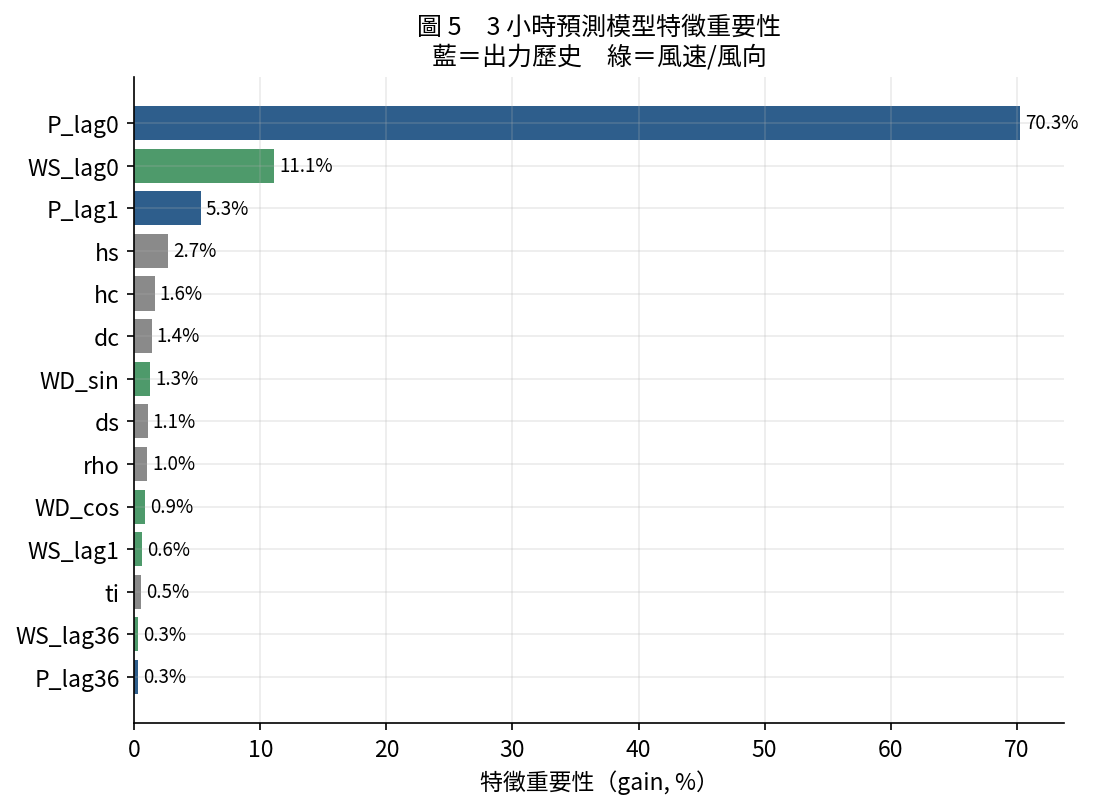
\includegraphics[width=\linewidth]{ml_project/power_forecast/figures/fc5_importance.png}
    {\scriptsize\centering 近時歷史（自我相關）$>$ 風速趨勢 $>$ 風向\par}
  \end{columns}
\end{frame}

% =====================================================================
\section{④ 預測方法}
% =====================================================================
\begin{frame}{④ 方法（一）：基準線、點模型、分位數}
  \footnotesize
  \textbf{基準線}：Persistence $\hat y{=}P(t)$；對稱 persistence（窗口）；Climatology（月$\times$時）。\\
  \textbf{點模型}：Ridge / XGBoost / \textbf{LightGBM}（樹模型吃下功率曲線非線性，全面最佳）。\\[4pt]
  \textbf{分位數迴歸}（pinball loss）：
  \[ L_\tau(y,\hat y)=\begin{cases}\tau(y-\hat y)& y\ge\hat y\\(\tau-1)(y-\hat y)& y<\hat y\end{cases} \]
  \textbf{CQR 保形校正}（可交換性下有涵蓋率理論保證）：
  \[ E_i=\max(\hat q_{lo}(x_i)-y_i,\ y_i-\hat q_{hi}(x_i)),\quad Q=\text{Quantile}_{\lceil(1-\alpha)(n+1)\rceil/n}(E) \]
  \[ \text{校正後}=[\hat q_{lo}(x)-Q,\ \hat q_{hi}(x)+Q] \]
\end{frame}

\begin{frame}{④ 方法（二）：Conformal 區間、遞迴軌跡、評分}
  \footnotesize
  \textbf{Conformal Prediction}（advanced）：以校準殘差 $r_i=|y_i-\hat y_i|$，
  \[ \hat q=\text{Quantile}_{\lceil(1-\alpha)(n+1)\rceil/n}(r),\ \alpha{=}0.1;\quad [\hat y-\hat q,\ \hat y+\hat q] \]
  \textbf{遞迴多步軌跡}：只訓一個 1 步（$t{\to}t{+}10$min）模型，回填展開至 144 步（24h），對照 Direct。\\[4pt]
  \textbf{評分公式}：
  \[ \text{Skill}=1-\frac{\text{RMSE}_{\text{model}}}{\text{RMSE}_{\text{persist}}},\quad
     \text{PICP}=\tfrac1n\sum\mathbb{1}[l_i\le y_i\le u_i] \]
  \[ W=\begin{cases}(u-l)+\tfrac{2}{\alpha}(l-y)& y<l\\(u-l)& l\le y\le u\\(u-l)+\tfrac{2}{\alpha}(y-u)& y>u\end{cases}
     \quad(\text{Winkler；越小越好}) \]
\end{frame}

% =====================================================================
\section{⑤ 建模架構與驗證}
% =====================================================================
\begin{frame}{⑤ 建模架構與驗證}
  \begin{columns}[T]
    \column{0.5\textwidth}
    \textbf{時序切分（不洩漏）}
    \begin{itemize}\footnotesize
      \item 家族一：訓練 $<$2020-06；測試 2020-06$\sim$2021-10
      \item 家族二：訓練 2016–18 / 驗證 2019 / 測試 2020–21
      \item CQR/Conformal 校準集：獨立用 2019 或 15\%
    \end{itemize}
    \column{0.5\textwidth}
    \textbf{驗證與超參數}
    \begin{itemize}\footnotesize
      \item 訓練期內 expanding-window TimeSeriesSplit 前推 CV
      \item LightGBM：\texttt{lr=0.03, leaves=45, subsample=0.8, n=250, seed=42}
      \item 固定種子、可續跑、完全重現
    \end{itemize}
  \end{columns}
  \vspace{4pt}
  \begin{block}{架構要點}\footnotesize
  一條「驗證 $\to$ 虛擬出力 $\to$ 特徵 $\to$ 模型選擇 $\to$ 評估」的獨立管線；各專案獨立資料夾、互不覆蓋，嚴格模擬「上線後預測未見過的未來」。
  \end{block}
\end{frame}

% =====================================================================
\section{⑥ 結果與應用價值}
% =====================================================================
\begin{frame}{⑥ 結果（一）：超短期點預測（正規化 nRMSE）}
  \centering\scriptsize
  \begin{tabular}{llcccccc}
    \toprule
    標的 & H & Persist. & Clim. & Ridge & XGB & \textbf{LGBM} & 勝 P.\\
    \midrule
    風速 & +1h & 0.149 & 0.479 & 0.141 & 0.138 & \best{0.1355} & +8.8\%\\
    風速 & +3h & 0.259 & 0.494 & 0.231 & 0.221 & \best{0.2176} & +16.1\%\\
    風速 & +6h & 0.372 & 0.502 & 0.311 & 0.297 & \best{0.2937} & +21.0\%\\
    發電 P & +1h & 0.284 & 0.655 & 0.267 & 0.252 & \best{0.2481} & +12.7\%\\
    發電 P & +3h & 0.456 & 0.665 & 0.396 & 0.366 & \best{0.3611} & +20.8\%\\
    發電 P & +6h & 0.624 & 0.671 & 0.490 & 0.455 & \best{0.4494} & +27.9\%\\
    \bottomrule
  \end{tabular}
  \vspace{4pt}
  \begin{columns}[c]
    \column{0.5\textwidth}
    \footnotesize 技術得分\textbf{隨時程放大}（+1h $\to$ +6h：+8\% $\to$ +28\%）——正是調度最需要幫助的區間。發電量比風速難（陡峭功率曲線放大中風速誤差）。
    \column{0.5\textwidth}
    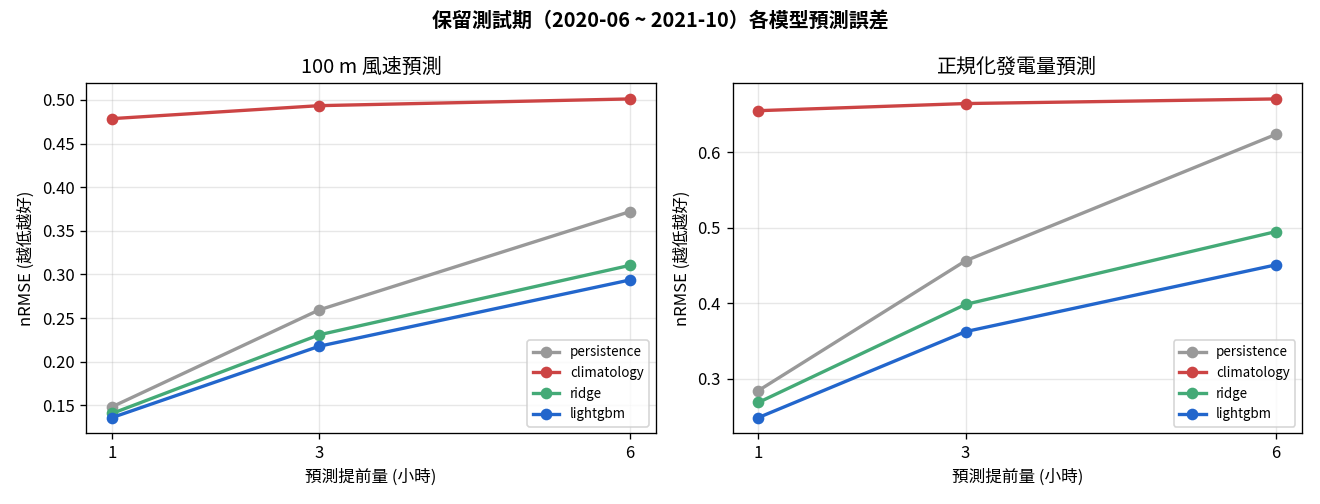
\includegraphics[width=\linewidth]{PW/figures/fig1_skill_by_horizon.png}
  \end{columns}
\end{frame}

\begin{frame}{⑥ 結果（二）：窗口能量（系統 A）與瞬時機率（系統 B）}
  \begin{columns}[T]
    \column{0.5\textwidth}
    \centering\scriptsize\textbf{系統 A：窗口平均（interval\_ge）}\\
    \begin{tabular}{lccc}
      \toprule H & $R^2$ & nRMSE & p10-p90\\ \midrule
      1h & \best{0.955} & 0.084 & 90.1\%\\
      3h & \best{0.914} & 0.114 & 88.8\%\\
      6h & \best{0.867} & 0.140 & 88.7\%\\
      24h & \best{0.712} & 0.185 & 70$\to$81\%\\
      \bottomrule
    \end{tabular}
    \column{0.5\textwidth}
    \centering\scriptsize\textbf{系統 B：瞬時區間（interval\_cl, CQR）}\\
    \begin{tabular}{lccc}
      \toprule H & p50 $R^2$ & 80\% & 90\%\\ \midrule
      1h & 0.904 & \best{79.8\%} & \best{91.4\%}\\
      3h & 0.784 & \best{80.2\%} & \best{90.5\%}\\
      6h & 0.652 & \best{80.9\%} & \best{90.1\%}\\
      \bottomrule
    \end{tabular}
  \end{columns}
  \vspace{3pt}
  \centering
  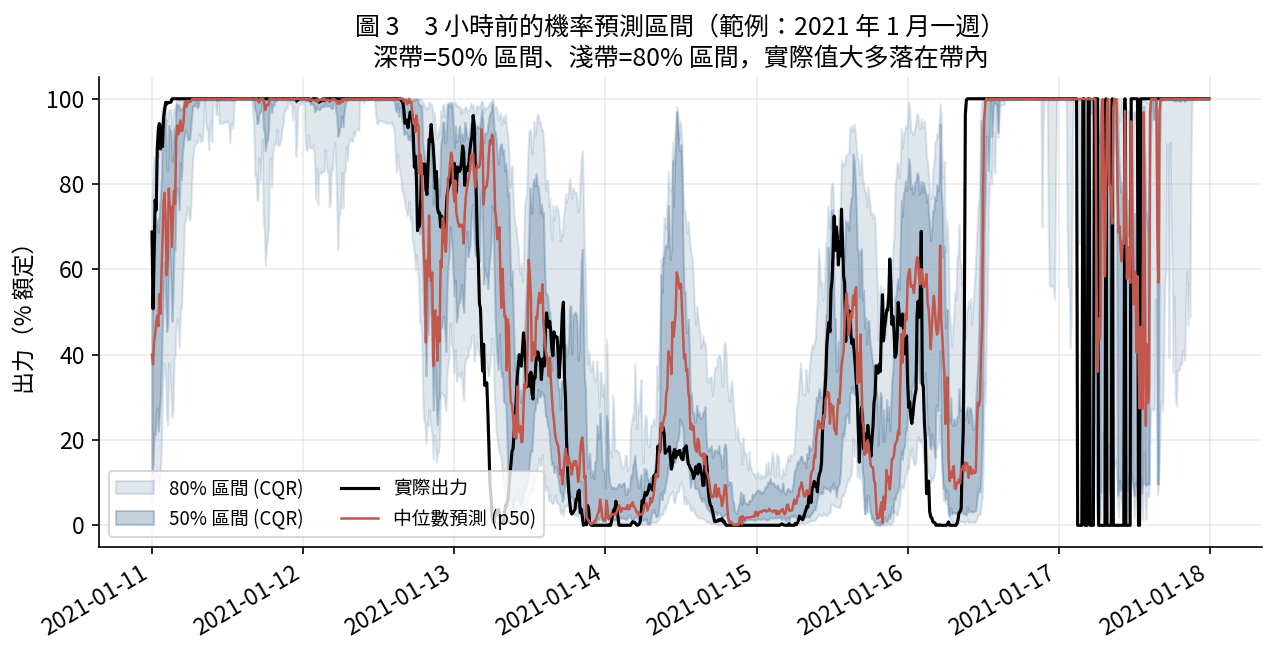
\includegraphics[height=3.5cm]{ml_project/power_interval_forecast_cl/figures/iv3_example_bands.png}
  {\scriptsize\par「會呼吸」的區間：轉折處變寬、穩定處收窄；80/90\% 校準到名目 $\pm$1pp。}
\end{frame}

\begin{frame}{⑥ 結果（三）：進階方法（NREL 5\,MW · 絕對 MW）}
  \centering\scriptsize
  \begin{tabular}{lccccc}
    \toprule
    時程 & Interval RMSE & Quantile RMSE & Recursive RMSE & Direct RMSE & 涵蓋率\\
    \midrule
    10min & 0.350 & 0.376 & \best{0.339} & 0.350 & 91.6\%\\
    1h & 0.650 & 0.684 & 0.775 & \best{0.648} & 92.9\%\\
    6h & 1.145 & 1.200 & 1.719 & \best{1.141} & 92.5\%\\
    24h & 1.600 & 1.674 & 1.996 & \best{1.593} & 92.5\%\\
    \bottomrule
  \end{tabular}
  \vspace{4pt}
  \begin{columns}[c]
    \column{0.5\textwidth}\footnotesize
    短時程遞迴最佳，但誤差累積使長時程劣於 Direct；Conformal 90\% 區間四時程涵蓋率穩定 91–93\%（單位 = 絕對 MW）。
    \column{0.5\textwidth}
    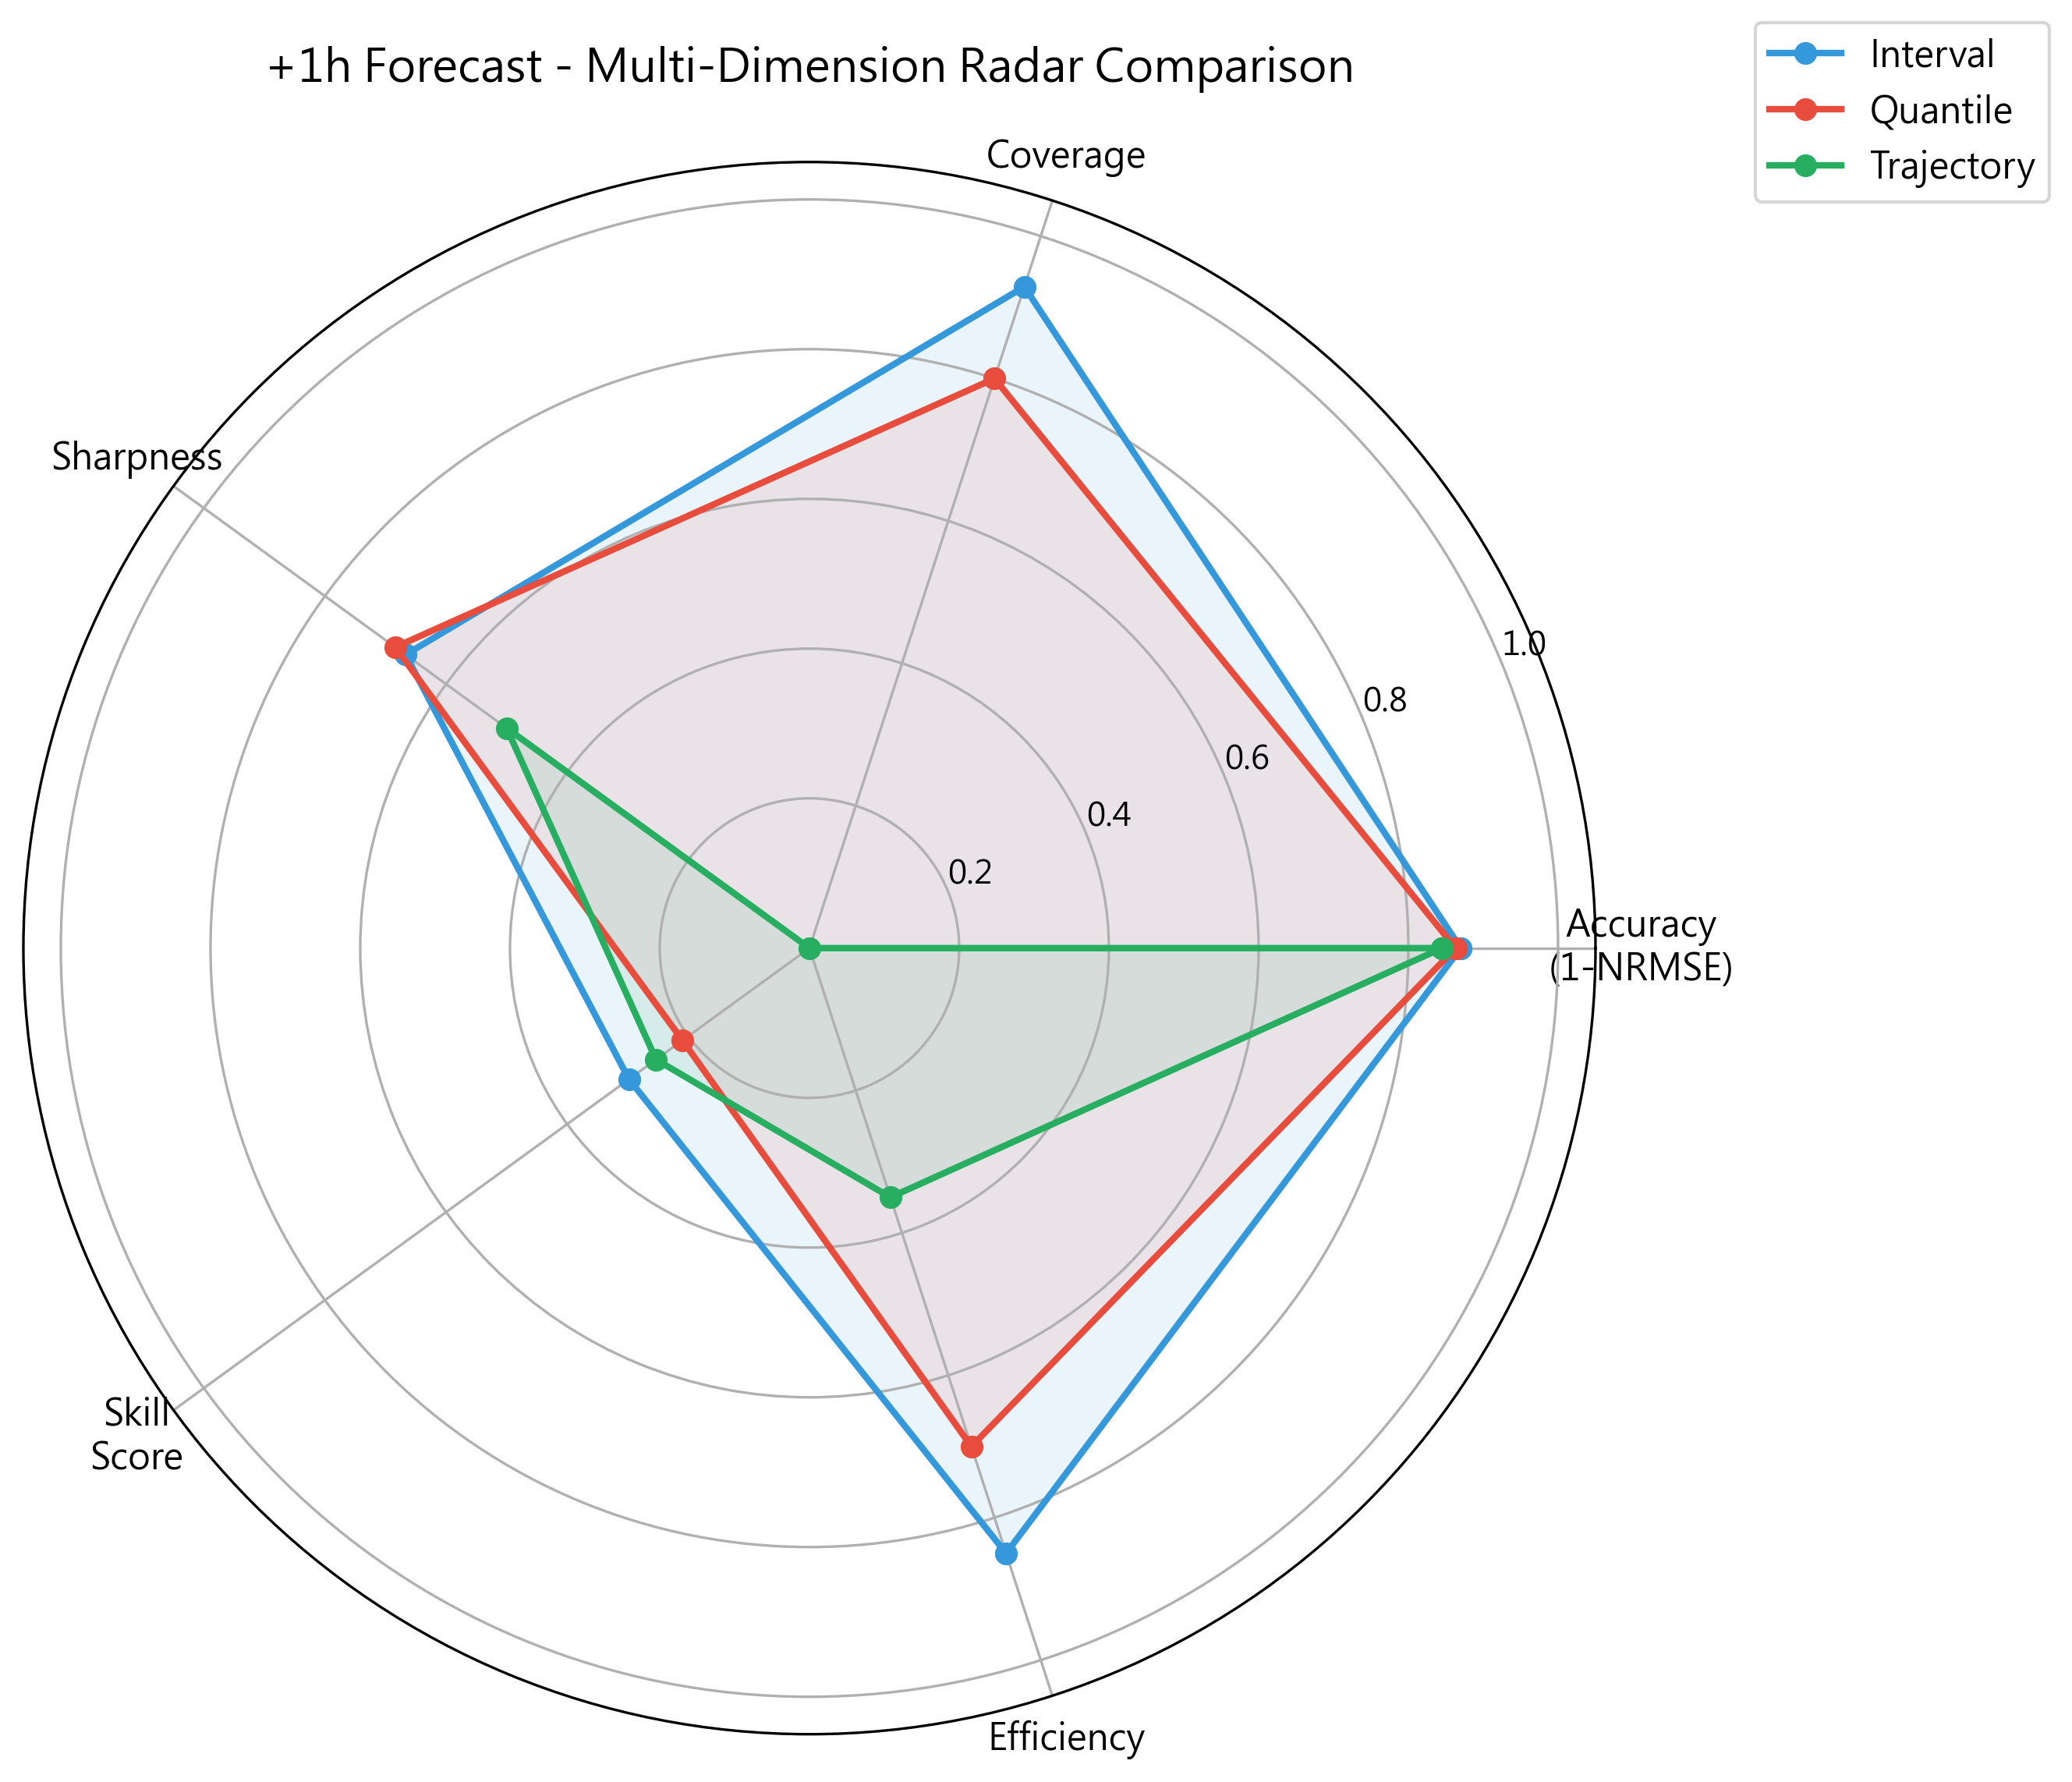
\includegraphics[width=\linewidth]{ml_project/advanced_forecasting/results/figures/compare_radar.png}
  \end{columns}
\end{frame}

\begin{frame}{⑥ 結果（四）：應用價值與經濟避險}
  \centering\footnotesize
  \begin{tabular}{lcc}
    \toprule
    項目 & 數值 & 專案\\
    \midrule
    日前 24h 能量 $R^2$ & \best{0.7209}（+28.2\%） & PW\_Interval\\
    100 MW 風場省下懲罰金 & \best{5{,}545 萬台幣}（避險 27.9\%） & PW\_Integrated\\
    +1h 劇烈爬升事件 ROC-AUC & 0.8706 & PW\_Integrated\\
    台電 15-min 即時轉供 $R^2$ & 0.9725 & PW\_Interval\\
    \bottomrule
  \end{tabular}
  \vspace{4pt}
  \begin{block}{定位}\scriptsize
  台幣金額建立在「虛擬出力 $\times$ 假設市場罰則」的試算，用來\textbf{示範預測改善的量級}，非實際財報。
  \end{block}
  \centering
  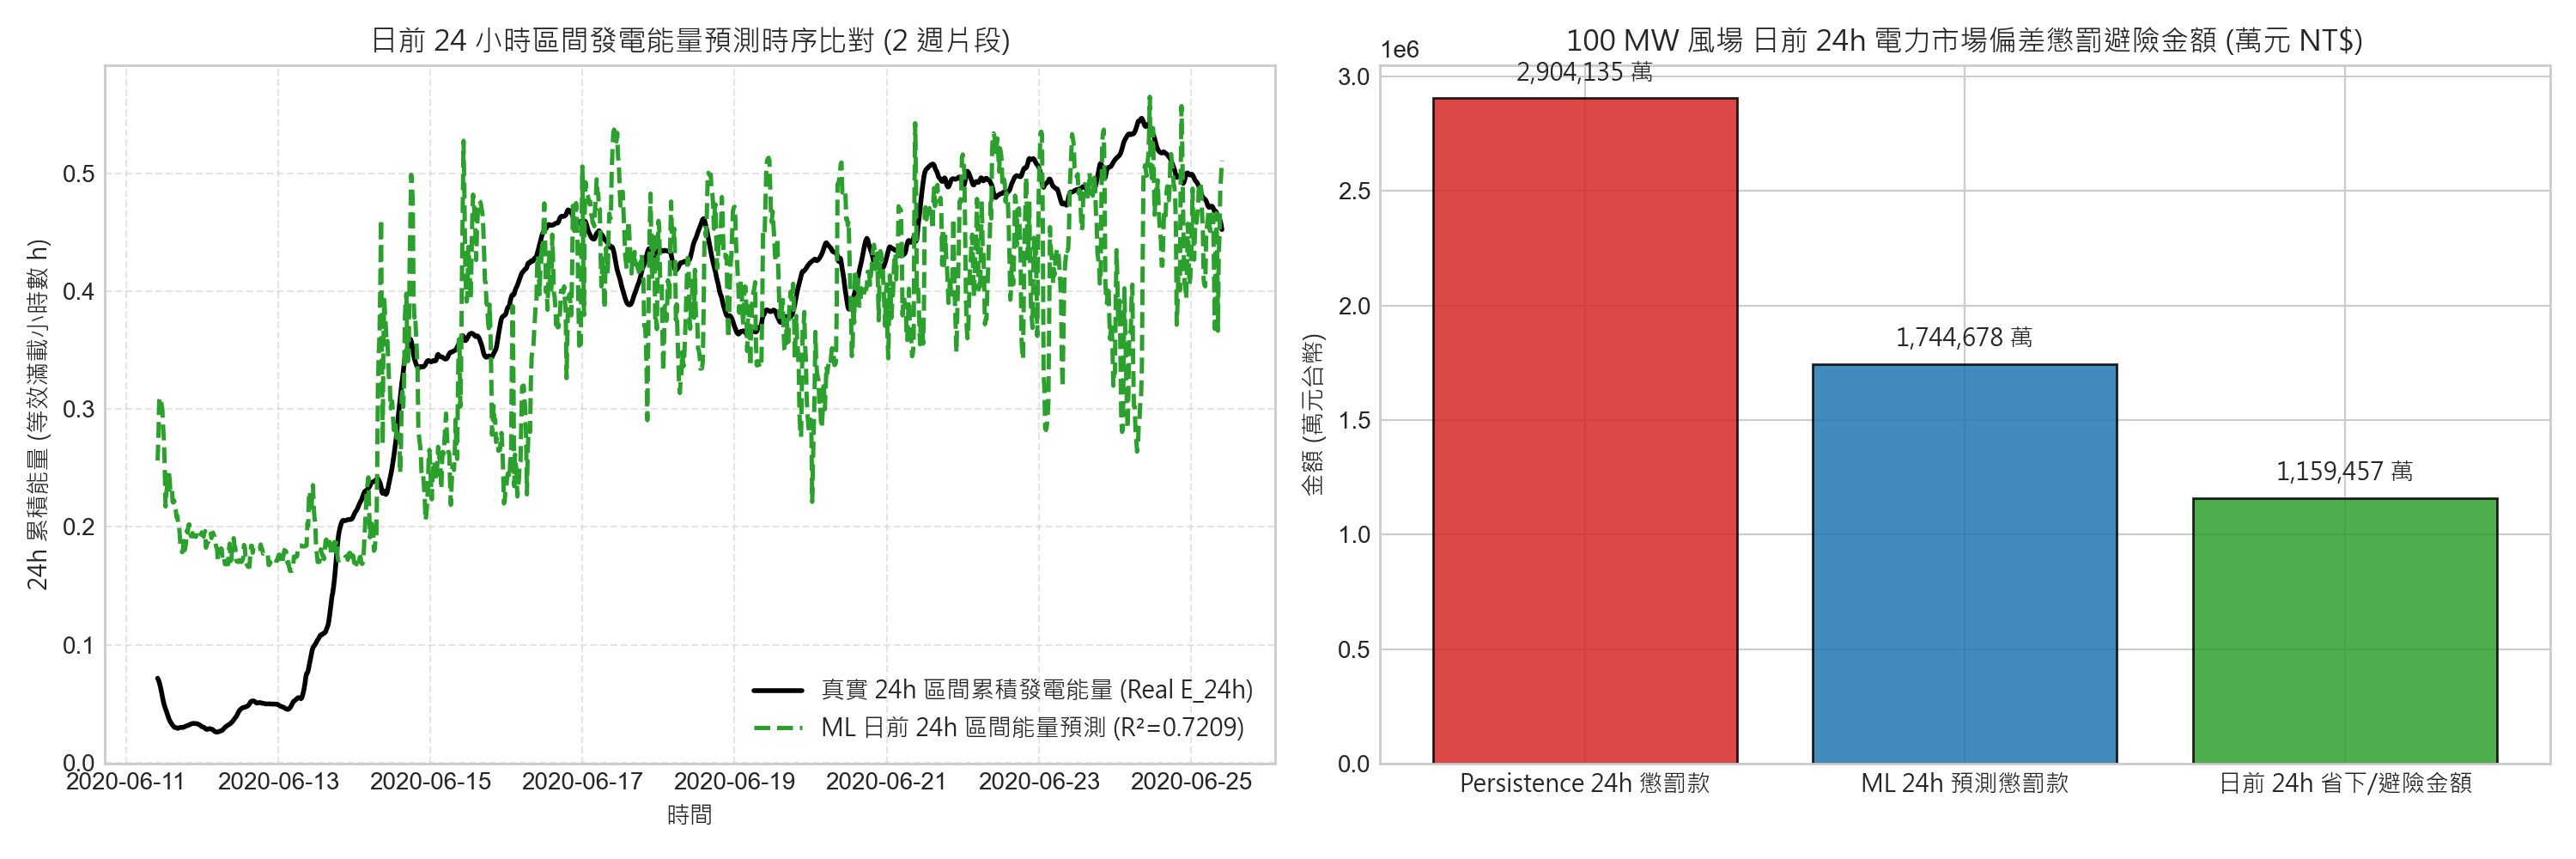
\includegraphics[height=3.2cm]{PW_Interval/figures/fig14_day_ahead_24h_settlement.png}
\end{frame}

\begin{frame}{附：湍流降尺度（不同層次的問題）}
  \footnotesize
  預測「當前 10 分鐘\textbf{湍流強度 TI $=\sigma/U$}」（關乎風機疲勞載重），60 個消融實驗：
  \begin{itemize}
    \item \textbf{最值得預測的方向是 TI}：只用風速 $R^2{\approx}0.14$，加完整特徵跳到 0.755（ML 加值 +0.66 最大）。
    \item \textbf{TI 幾乎完全由風向決定}：8 特徵模型中四個風向分量佔重要性 \textbf{90\%}（單 \texttt{WD\_97\_cos} 57\%）。物理：不同風向的上風地表粗糙度差異巨大。
    \item \textbf{用 8 特徵打敗 17 特徵}：熱力與 \texttt{veer} 特徵被證實有害；精簡 \texttt{core8} 測試 $R^2{=}0.781$（天花板 0.99）。
  \end{itemize}
\end{frame}

% =====================================================================
\section{限制與總結}
% =====================================================================
\begin{frame}{誠實限制（七專案共通）}
  \begin{enumerate}\footnotesize
    \item \textbf{虛擬出力非實測}：尾流/可用率/機型皆假設，可用台電公開 CF 校準。
    \item \textbf{理想切出風速}：25 m/s 硬切，實際風機有遲滯，極端強風彈跳在真實中較平緩。
    \item \textbf{短時程機率區間略保守}：零/額定「點質量」讓低分位較難校準（80/90\% 不受影響）。
    \item \textbf{逐時日前仍需 NWP}：塔只有「過去到現在」，$>$6h persistence 逼近長期平均而失效；日前 48h 需接 CWA/ERA5 數值天氣預報做偏差校正。
  \end{enumerate}
\end{frame}

\begin{frame}{一頁總結}
  \begin{block}{一座測風塔 + 一條物理功率曲線 = 一座「虛擬風場」}
  \footnotesize
  以六階段管線（QC $\to$ 虛擬出力 $\to$ 特徵 $\to$ 方法 $\to$ 驗證 $\to$ 結果）：
  \begin{itemize}
    \item 這是個\textbf{容量因數 45\%} 的優質離岸站點；
    \item LightGBM 在 0–6h \textbf{全面打敗 persistence}（+8\% $\sim$ +28\%，時程越長優勢越大）；
    \item 改預測\textbf{窗口能量}後 3h $R^2$ 由 $\sim$0.79 跳到 0.91；日前 24h 能量 $R^2{=}0.72$；
    \item \textbf{機率區間}（CQR）在 80/90\% 校準到名目 $\pm$1pp，可直接用於備轉容量規劃；
    \item \textbf{advanced\_forecasting} 用 NREL 5\,MW 絕對量示範 Conformal/Quantile/Trajectory；
    \item 湍流降尺度證明 \textbf{TI 幾乎完全由風向決定}（8 特徵 $R^2{=}0.78$）。
  \end{itemize}
  要再往日前 48 小時，才需要接氣象署數值預報——那是測風塔的物理極限之外。
  \end{block}
  \centering\vspace{2pt}
  {\footnotesize\textcolor{accent}{\rule{0.9\textwidth}{0.4pt}}\\ 謝謝指教}
\end{frame}

\end{document}
